\section{Final System Architecture and Design}

\subsection{System Architecture}
When we were planning our project, we decided upon incorporating the MVC (Model-View-Controller) architecture. We were all familiar with it and it seemed like a good option based on our project's needs. We started off strong, but it slowly became muddled as time went on in the project. Particularly, the Model and View aspects blended more than they should have within our project, simply because we were focused on getting the assignment requirements complete, and the most convenient way for us resulted in this. However, we did not completely stray from it, and still made use of our Controller classes to the best of our abilities.

\subsection{Libraries, Modules \& Packages}
\label{sec:libs/mods/packs}
We made use of a lot of helpful tools. The libraries we used included ReactJS for HTML/JavaScript, Lucide for icons, Material UI for React components, bootstrap for css, and testing-library/react. One module we used was dotenv for loading environment variables.
Lastly, a package we used the Firebase SDK.

\subsection{Coding Standards}
\subsubsection{Comments}
General code comments were placed above the lines of code they pertained to, never on the same line. Comments were meant to be clear, concise and in plain-english.

\subsubsection{Function Headers}
For Java game logic functions, we used consistent headers (in plain-english) including:
\begin{itemize}
    \item [--] Input: what the function received as input.
    \item [--] Output: what the function produced.
    \item [--] Purpose: what the function accomplished.
\end{itemize}

\subsubsection{Variables}
Following the same standard across all of our code, all variables were camel case and singular. 

\subsubsection{Database}
\label{sec:database}
Our initial plan was to use the relational SQL database management system, MySQL. However, during Sprint 1, we ran into issues with sharing a local instance of the database, so we decided to migrate to using a cloud-based No-SQL database called Firestore from Google Firebase. This was relatively easily implemented into our project.

With the original MySQL database, we planned for our table names to be Pascal case and singular. The primary keys were camel case followed by 'ID'. The foreign keys were also camel case with a descriptor followed by 'FK'.

In our ERD, the different tables were represented as rectangles and the fields were represented as ovals. In addition, primary keys were bolded and underlined, along with having an @ symbol in the front. Foreign keys were marked by a \# in front. Lastly, composite keys were marked like primary keys, but with an additional \# after the @ symbol. This is the ER diagram of our original database: 

\begin{figure}[hbt!]
    \centering
    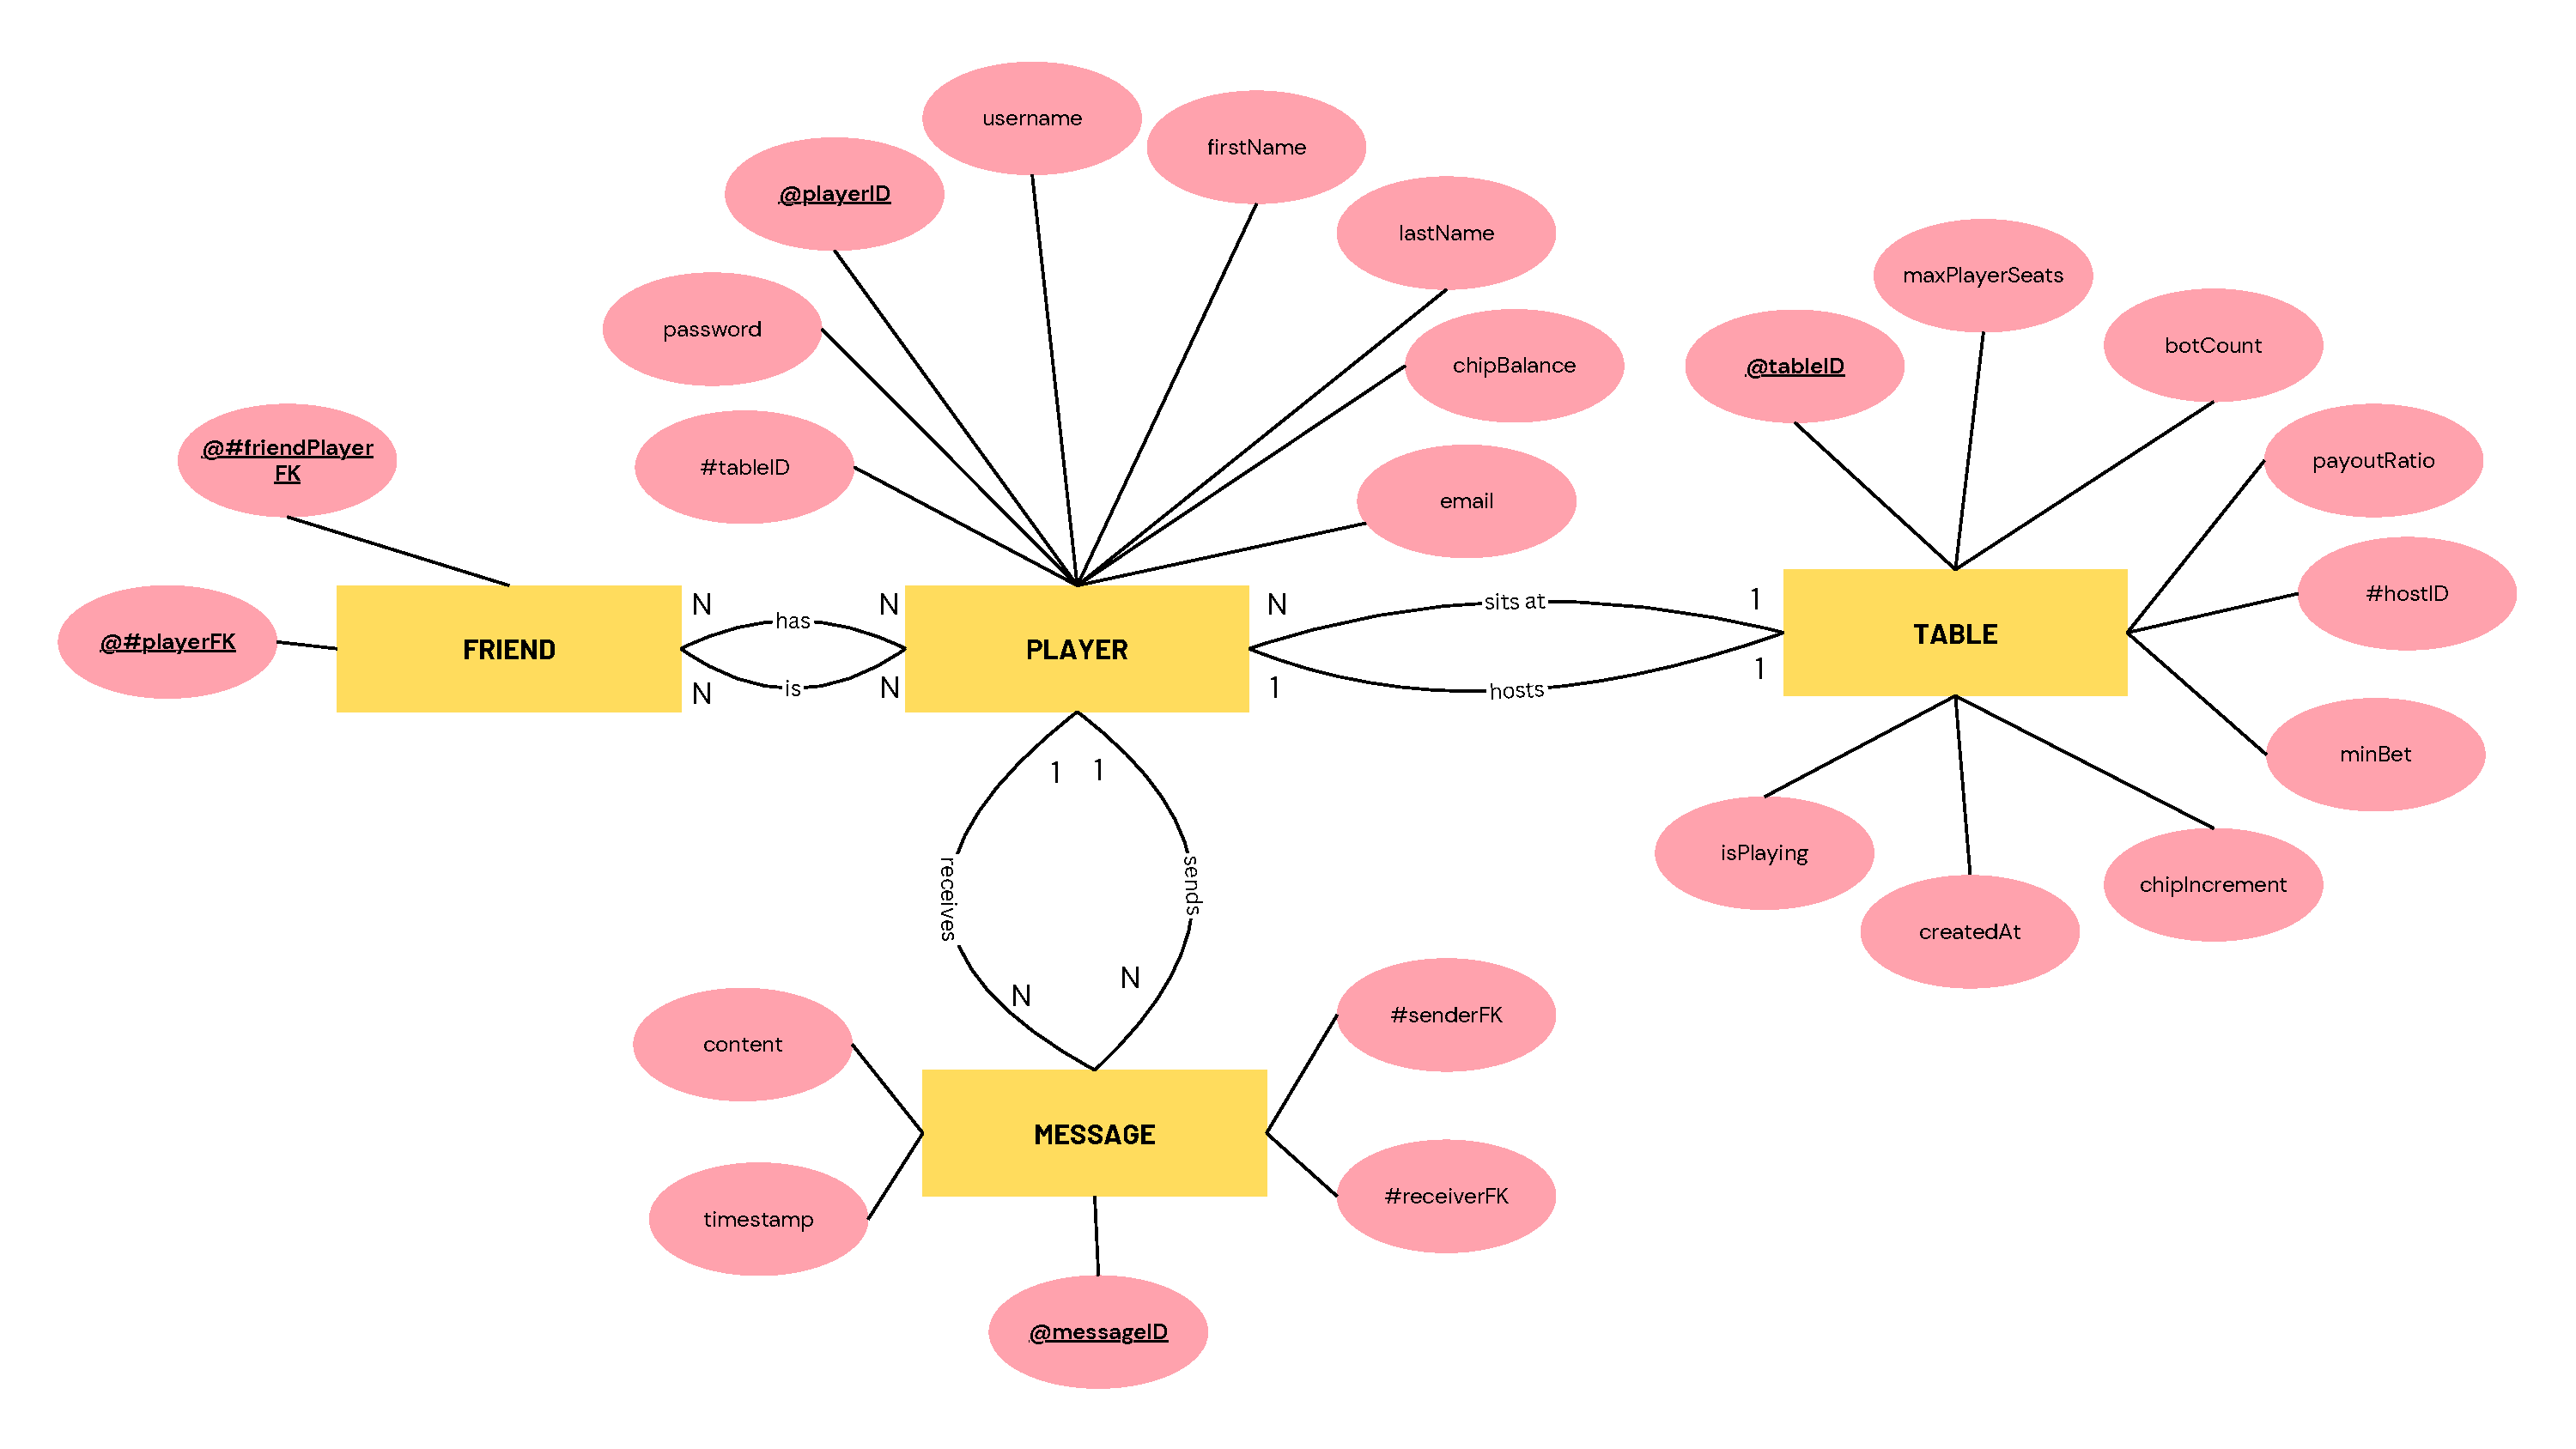
\includegraphics[width=1.0\linewidth]{figures/SE Database ERD.pdf}
    \caption{ERD for our original database plan.}
    \label{fig:ERD}
\end{figure} 

Since we switched from SQL to NoSQL, we also changed the naming conventions. We went from having tables to collections, and our collections were generally camelcase and plural. The documents within a collection had auto-generated identifiers, and the fields within documents were camelcase.

The model for our NoSQL database appeared similar to our original, but there were noticable changes. Collections were made as rectangles and fields as ovals. Even though there are not technically ''relationships`` in NoSQL databases, we included lines between collections to show when the equivalent to a foreign key was propagated from one collection to another. Subcollections were marked in purple. To prevent clutter and confusion, we left out the individual fields of these subcollections, as their names provided a satisfactory description of what they contained. Here is the updated diagram of our database:

\begin{figure}[hbt!]
    \centering
    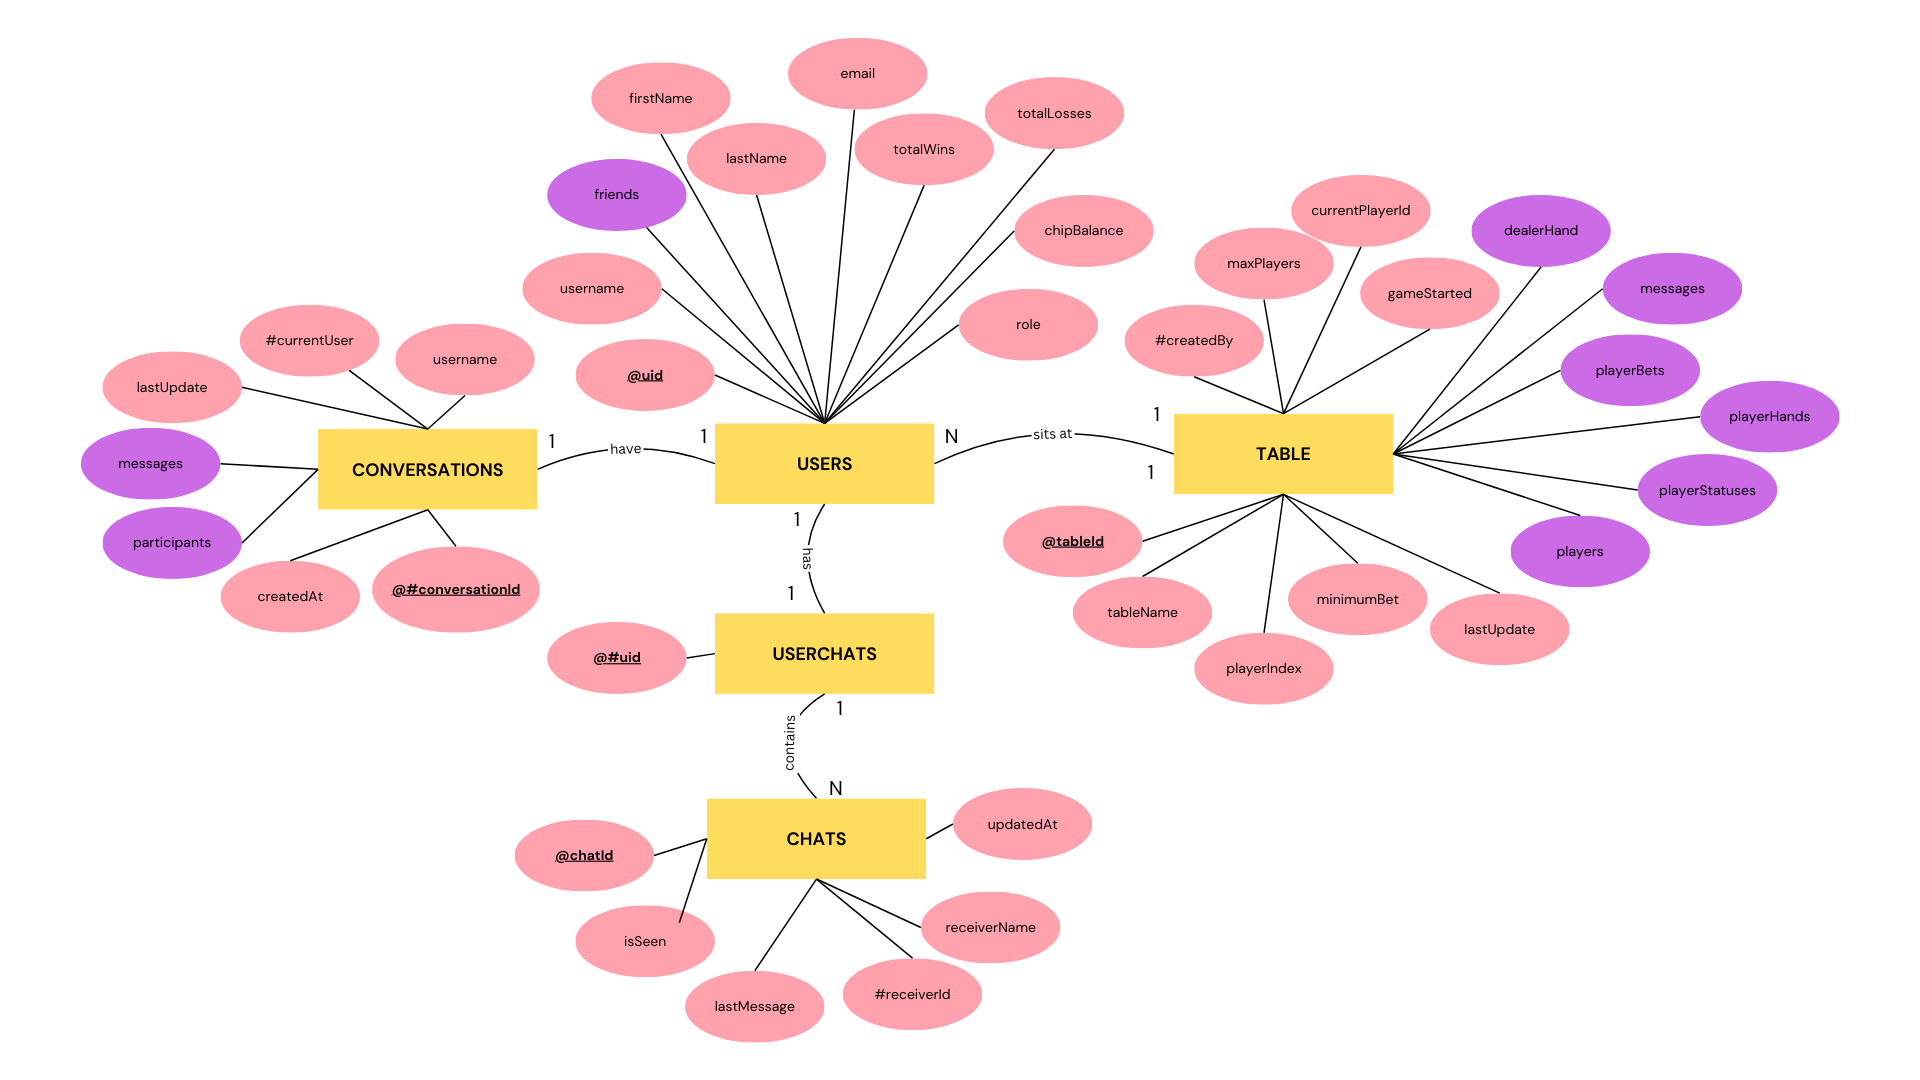
\includegraphics[width=1.0\linewidth]{figures/NoSQL_Database_Model.png}
    \caption{NoSQL database model.}
    \label{fig:ERD}
\end{figure}


\pagebreak

\subsection{Technologies Used}

\subsubsection{Languages}
As stated earlier, we initially used SQL for our database, but because of the issues mentioned in the \hyperref[sec:database]{Database} section, we ended up using NoSQL. 

For the language to run our game logic, we chose Java as we were familiar with it, and it seemed a logical choice as an object-oriented programming language. For our web UI we used Javascript and HTML, which was supplemented by ReactJS as mentioned \hyperref[sec:libs/mods/packs]{here}.

Here is our initial UML class diagram that outlined our plan of the major classes in our game logic:  

\begin{figure}[hbt!]
    \centering
    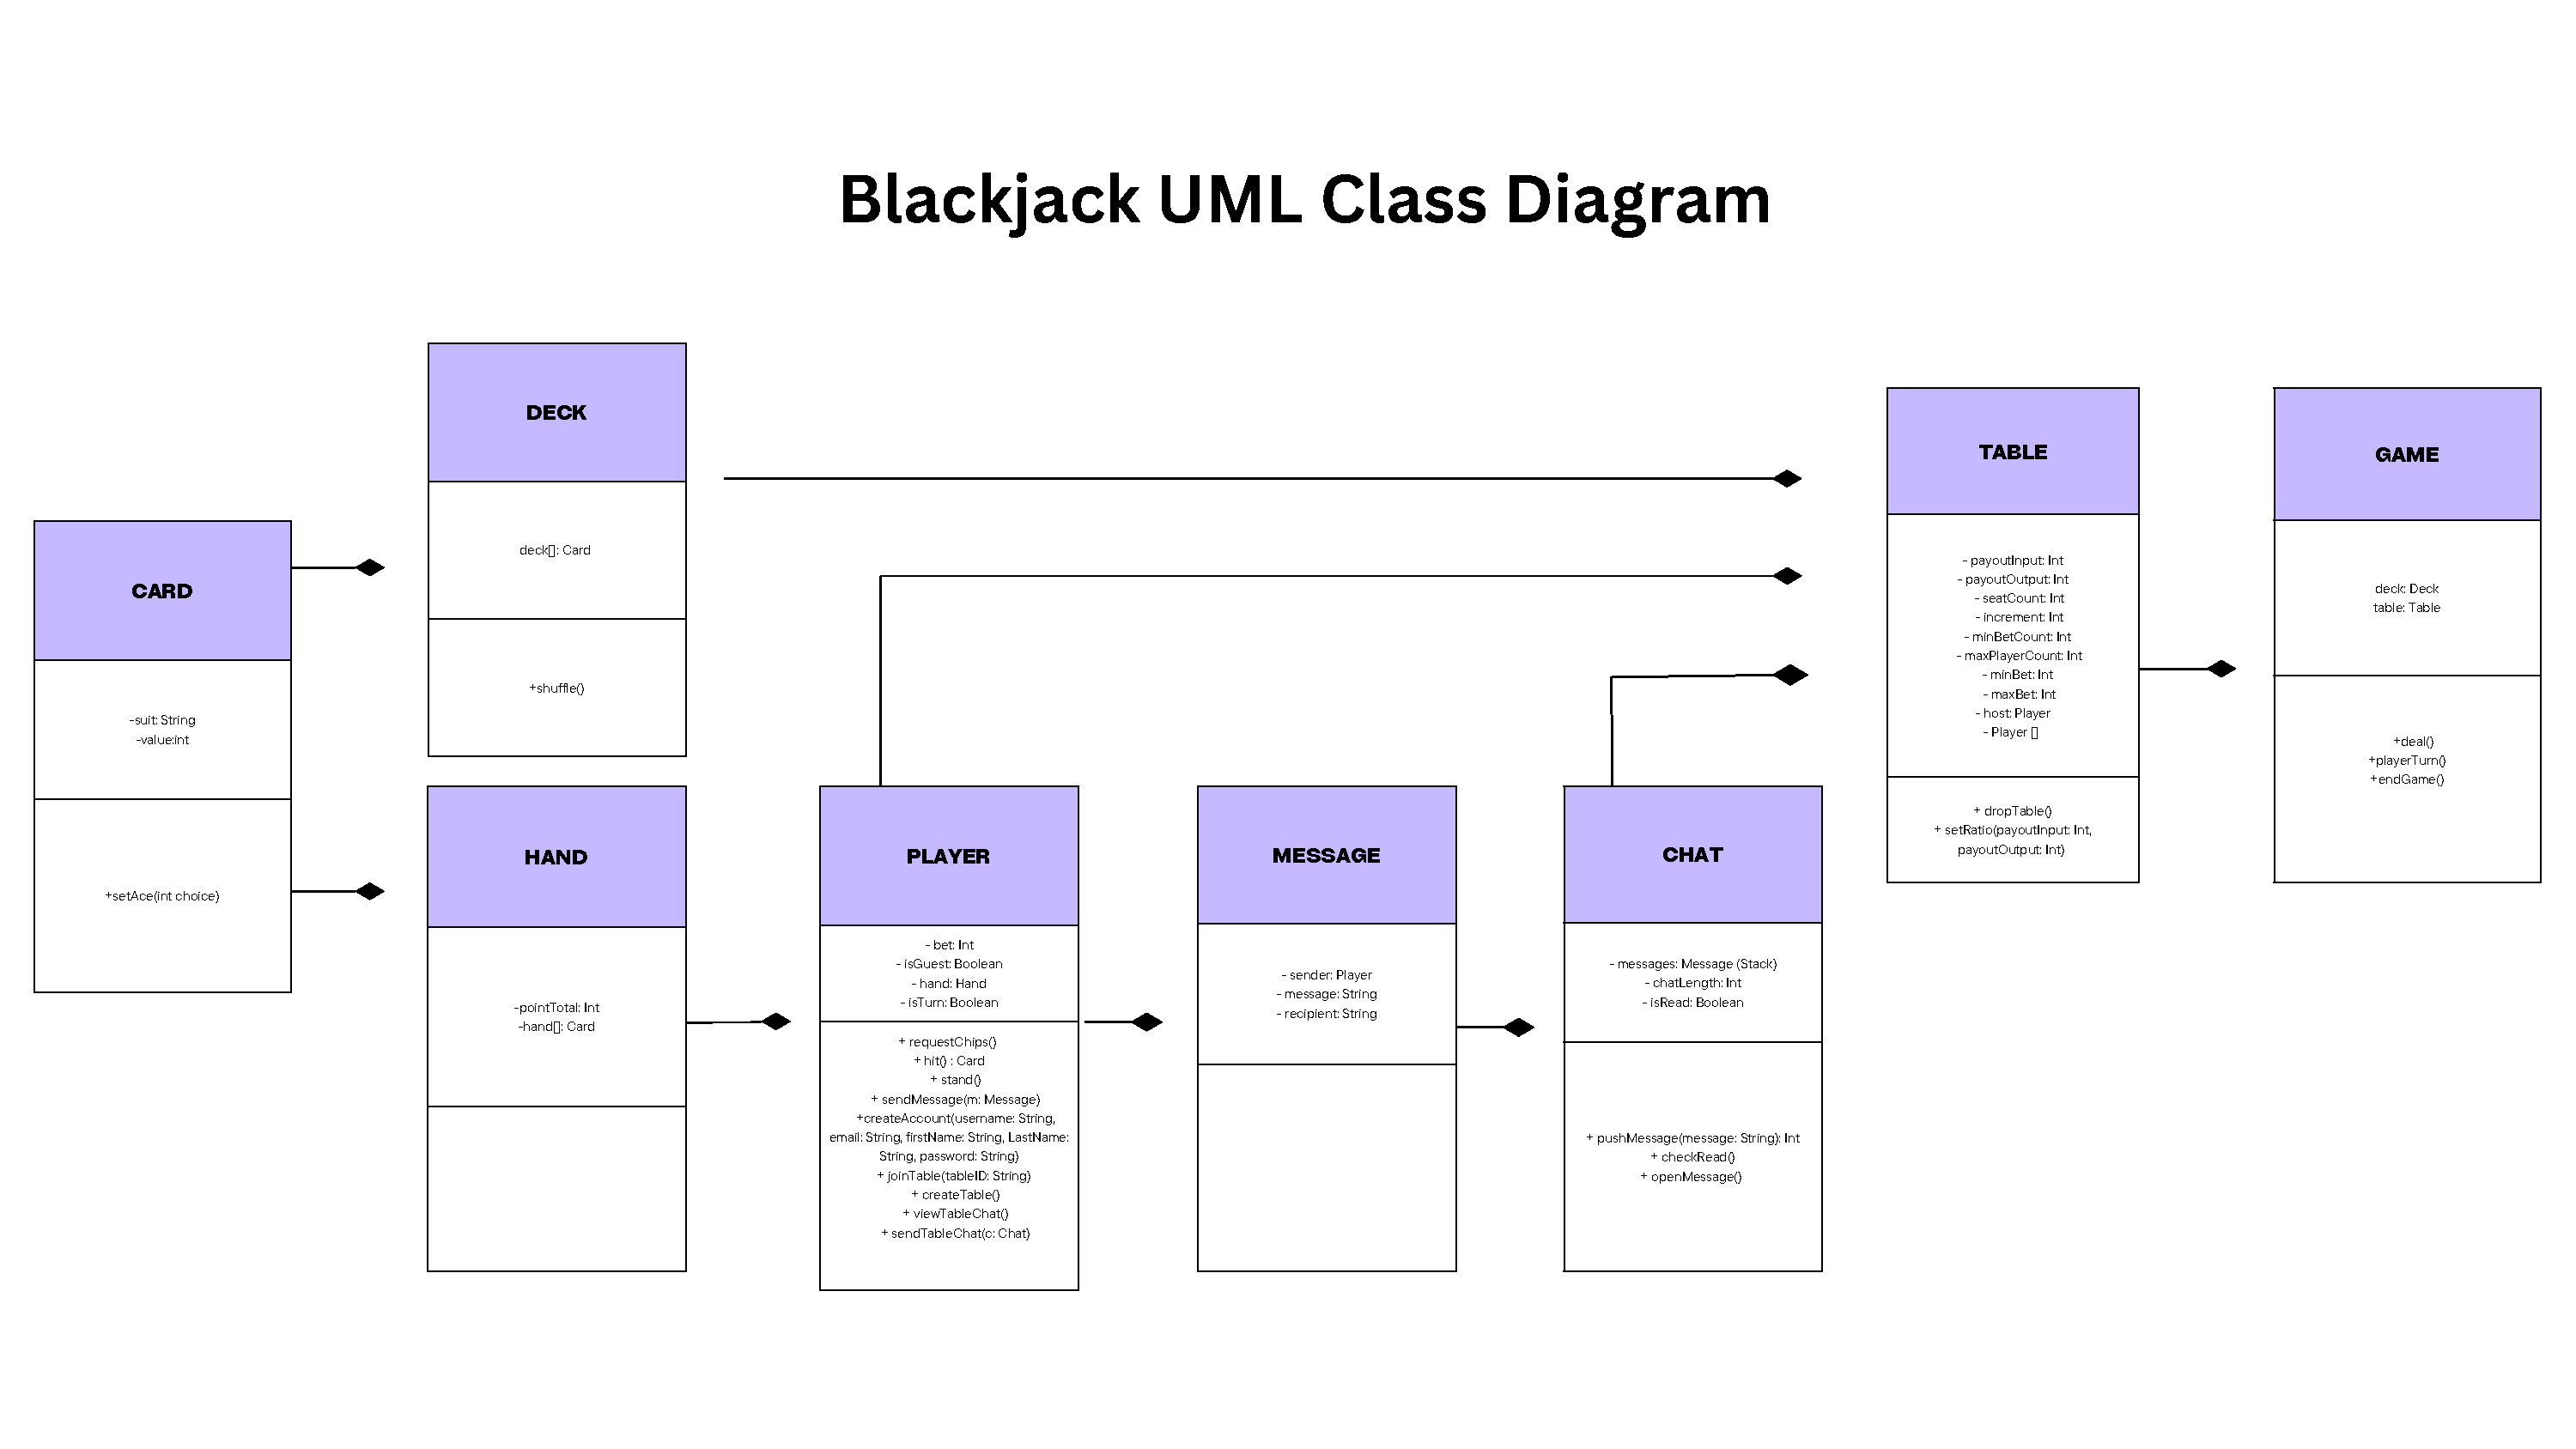
\includegraphics[width=0.8\linewidth]{figures/UML Diagram Whiteboard.pdf}
    \caption{UML diagram of major classes and relations.}
    \label{fig:UML}
\end{figure}

Below is our updated UML class diagram:
% PLACE UPDATED DIAGRAM

\pagebreak

\subsection{UI Mockups}
Here are some of the initial UI designs for our project:

\begin{figure}[hbt!]
    \centering
    
\includegraphics[width=0.5\textwidth]{figures/Blackjack.png} \\
    \caption{This is the UI mockup for the logo of the app (illus. Emma Heiser)}
    \label{fig:logo}
\end{figure}

\begin{figure}[hbt!]
    \centering
    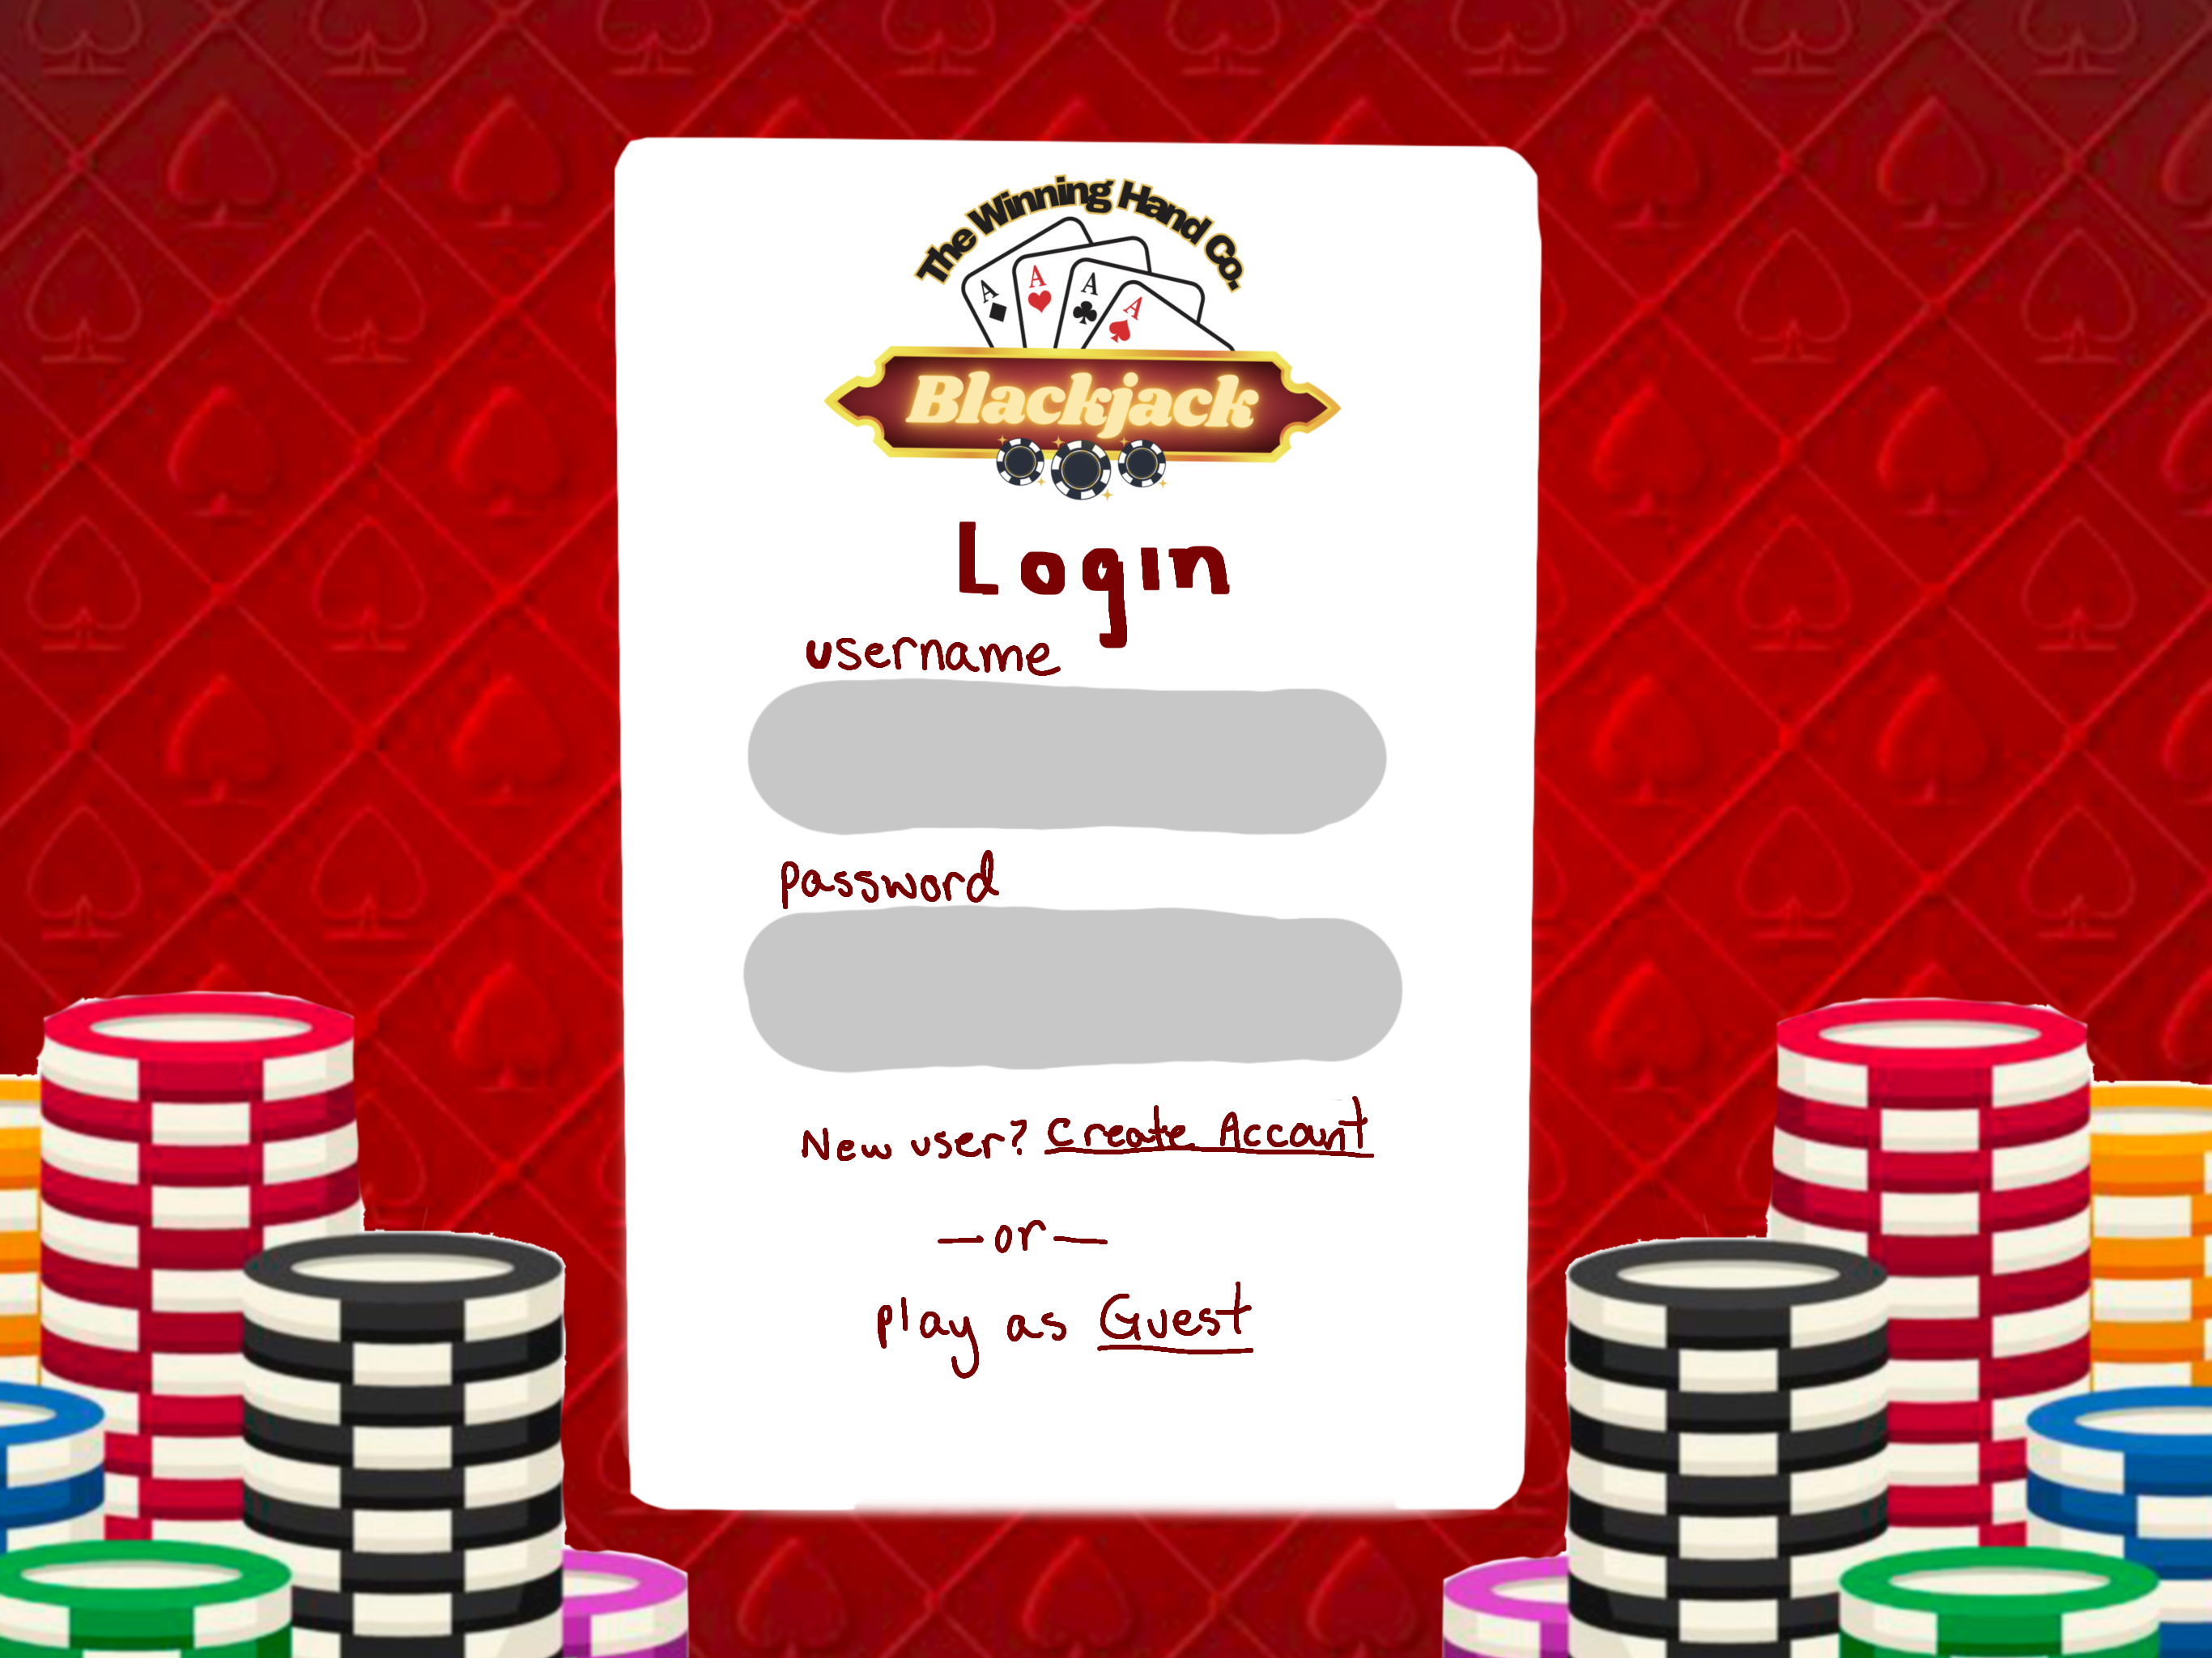
\includegraphics[width=0.75\linewidth]{figures/login.png}
    \caption{This is a UI mockup of the login screen (illus. Emma Heiser)}
    \label{fig:login}
\end{figure}

\begin{figure}[hbt!]
    \centering
    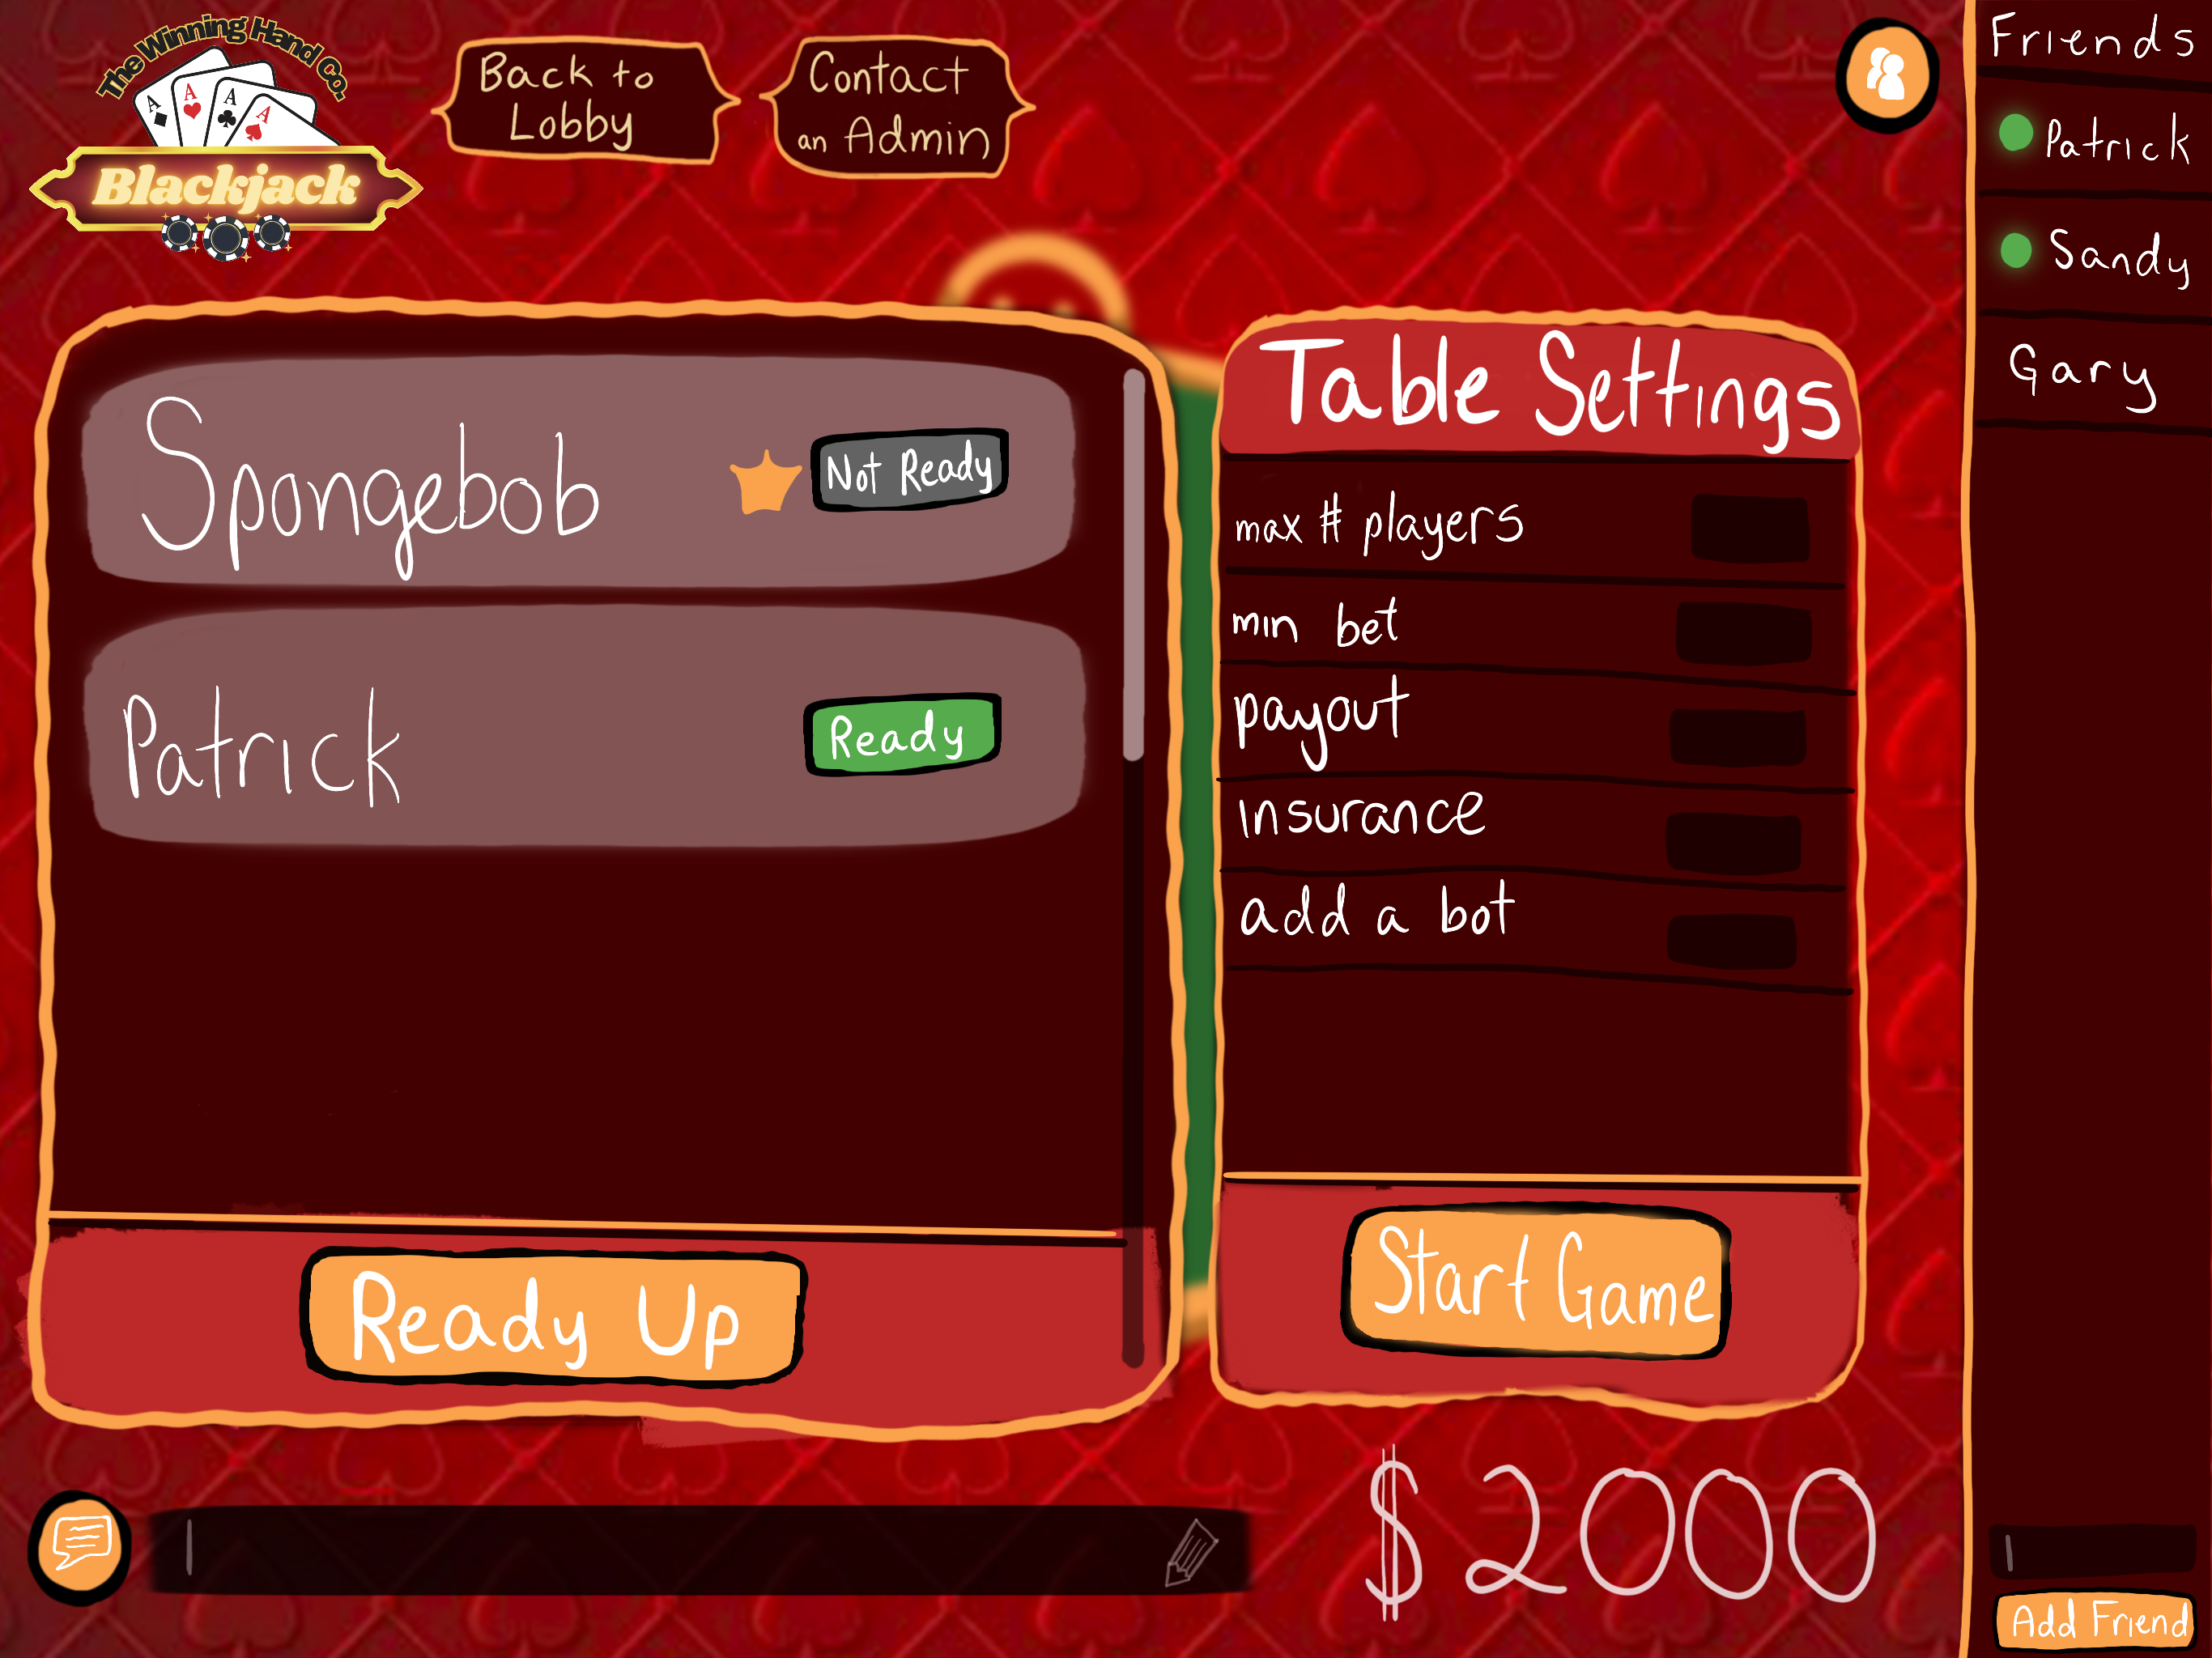
\includegraphics[width=0.75\linewidth]{figures/at-table.png}
    \caption{This is the UI mockup of creating a table (illus. Emma Heiser)}
    \label{fig:table}
\end{figure}

\pagebreak

\begin{figure}[hbt!]
    \centering
    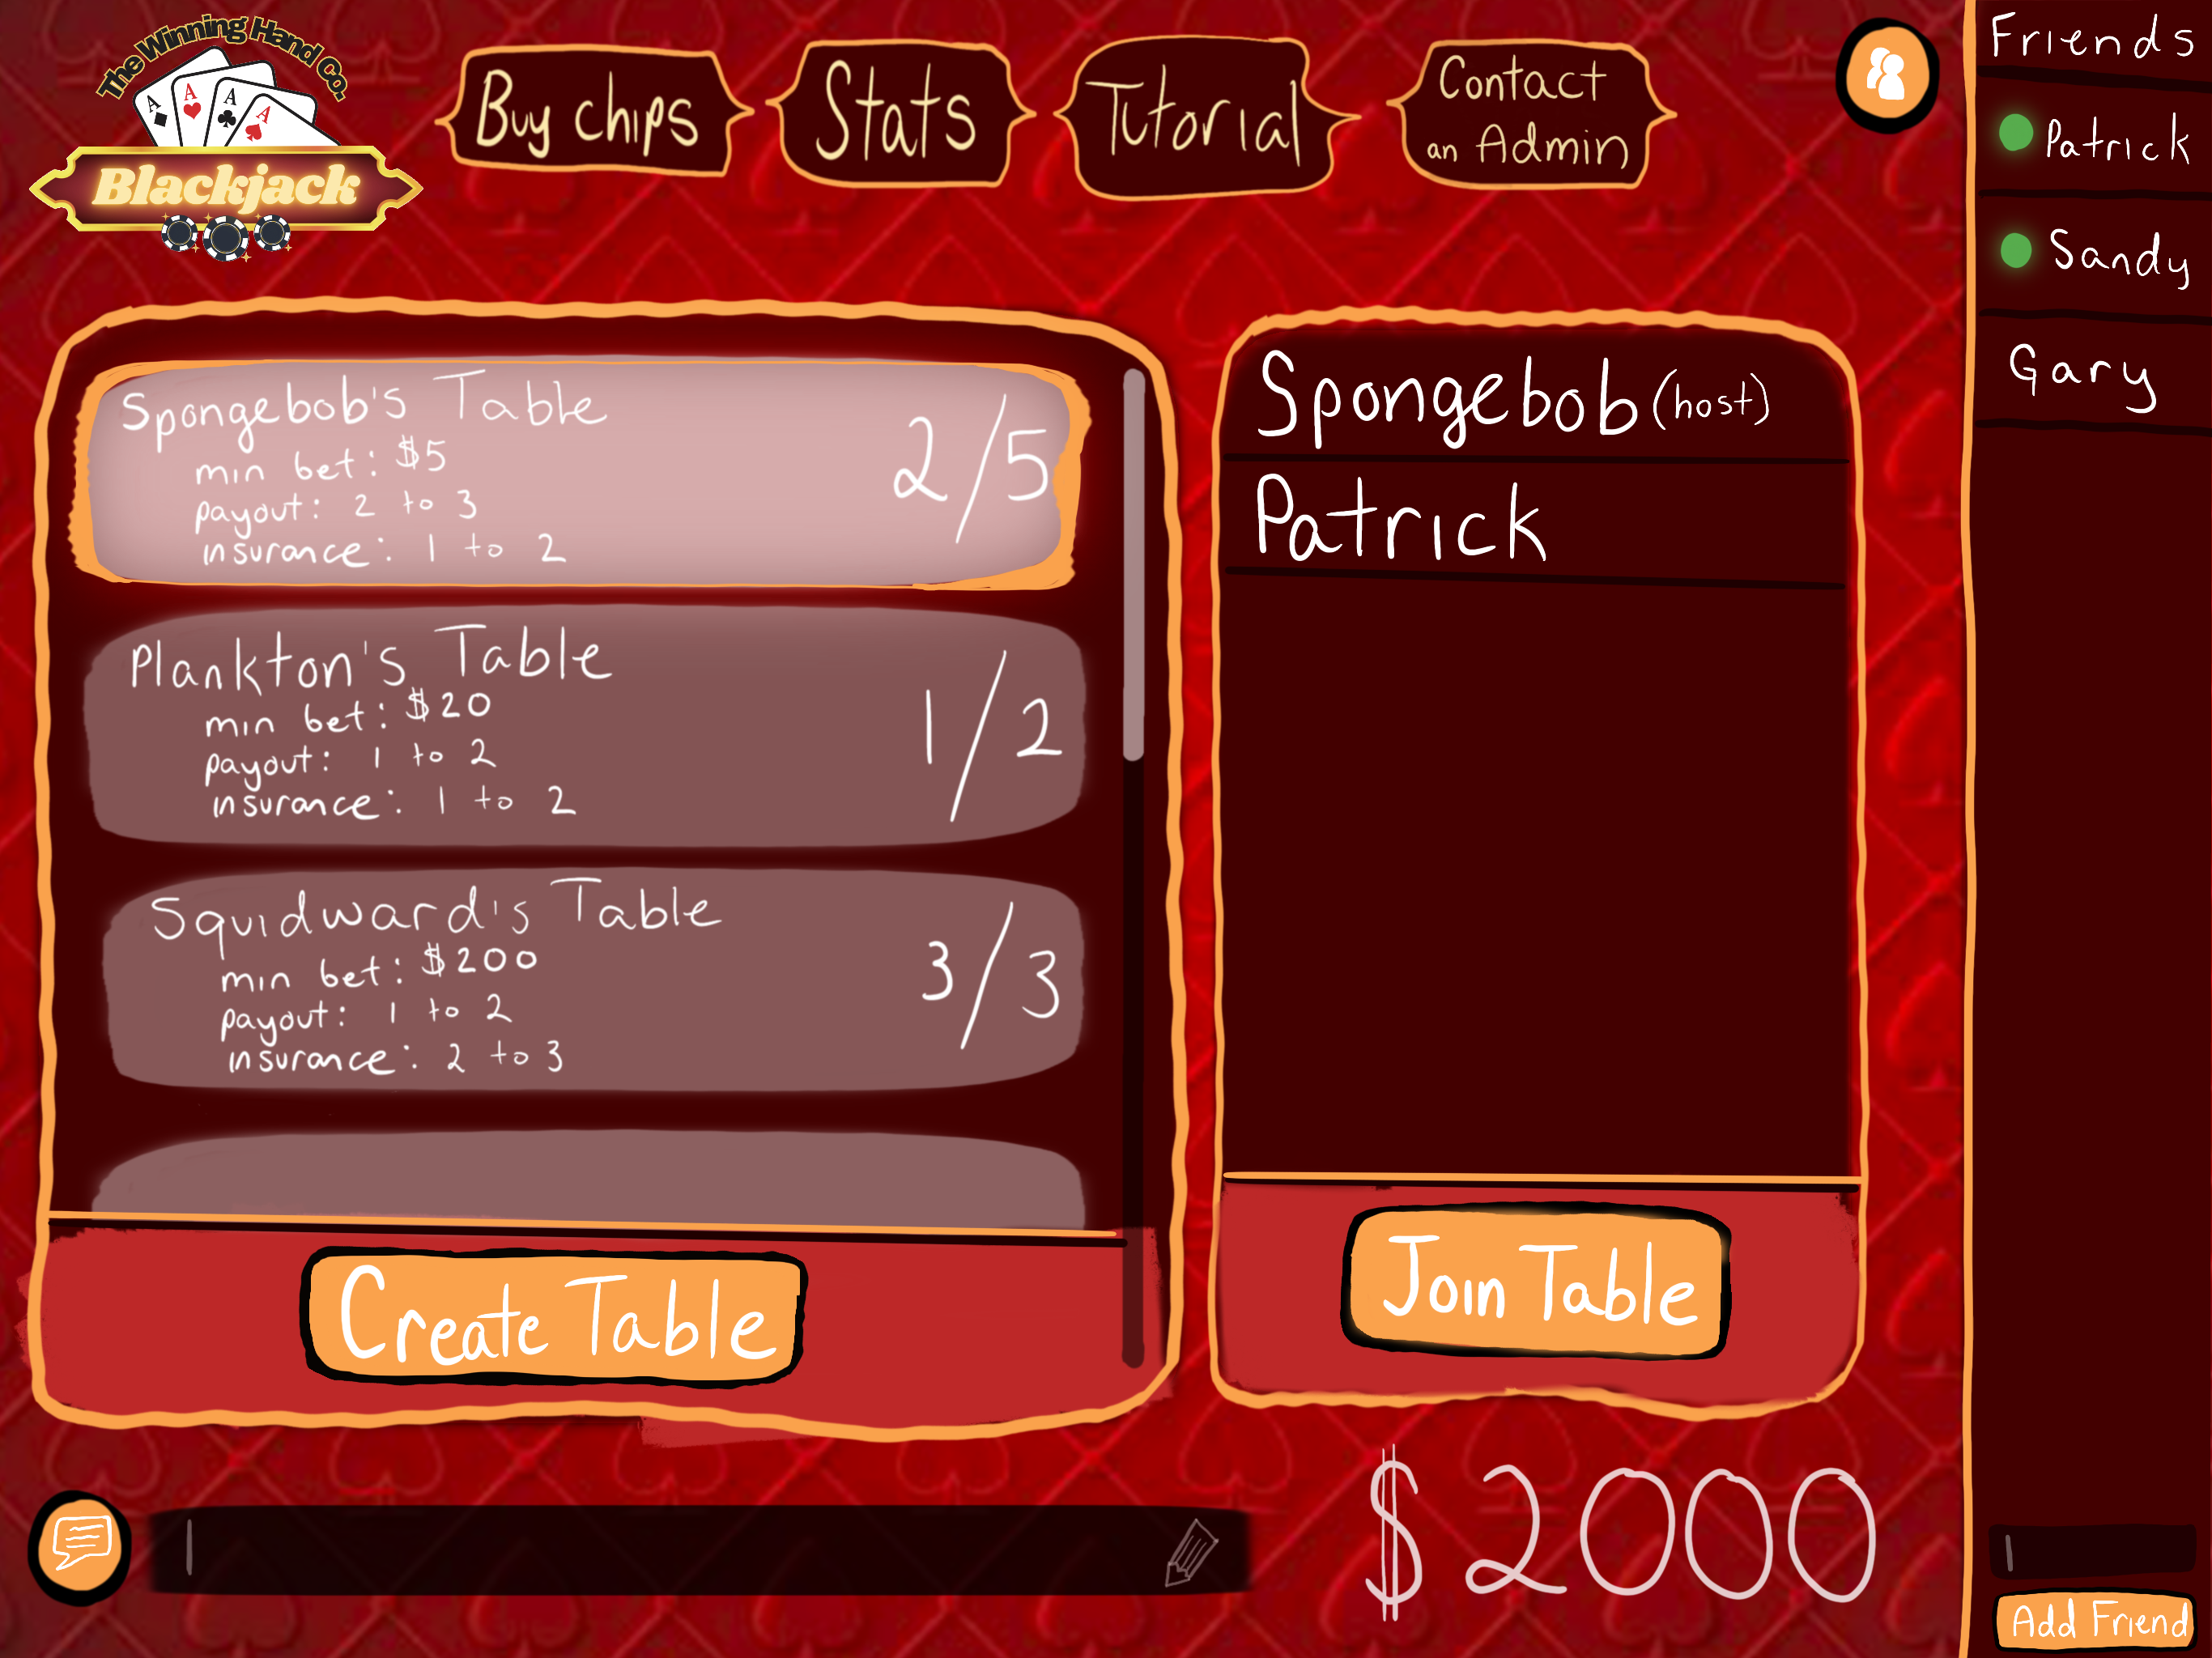
\includegraphics[width=0.75\linewidth]{figures/lobby.png}
    \caption{This is the UI mockup for the lobby where players can see available tables (illus. Emma Heiser)}
    \label{fig:lobby}
\end{figure}

\begin{figure}[hbt!]
    \centering
    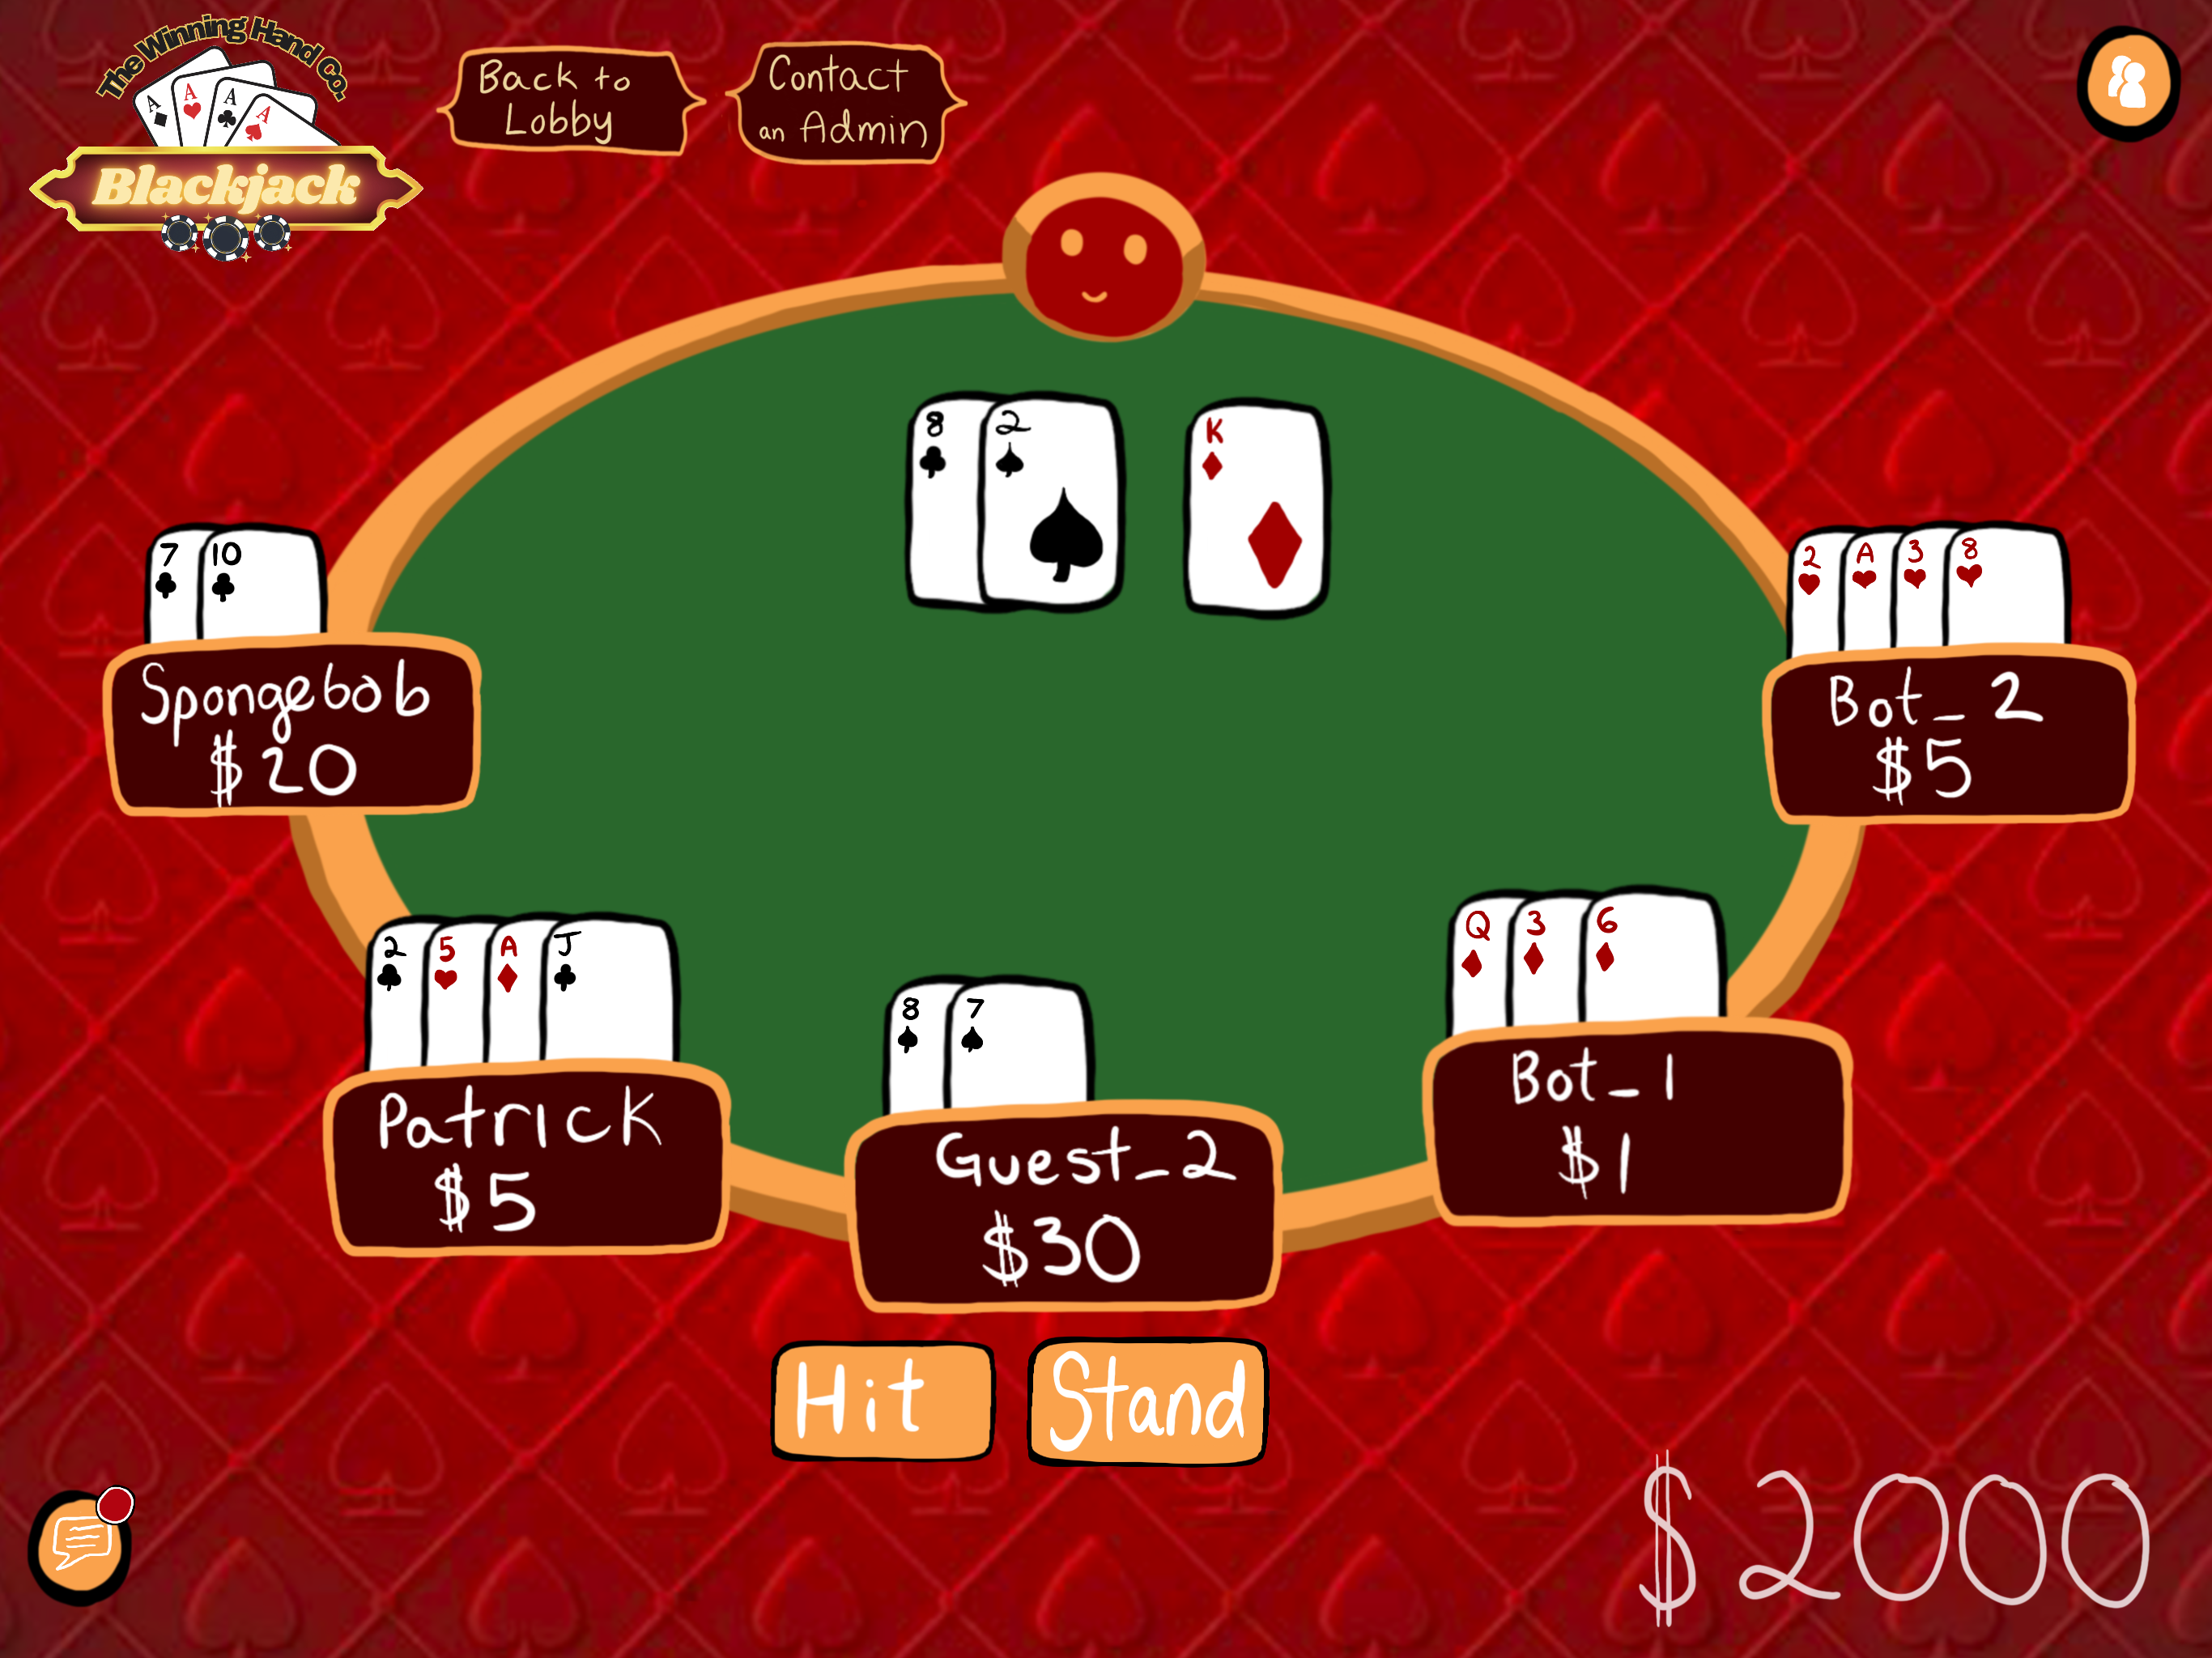
\includegraphics[width=0.75\linewidth]{figures/in-game.png}
    \caption{This is the UI mockup of the game being played at a table (illus. Emma Heiser)}
    \label{fig:game}
\end{figure}

\pagebreak
